% AUTHOR ===================================================================================================================
% Manuel Lippert (GitHub: ManeLippert (https://github.com/ManeLippert))
% ==========================================================================================================================

% PREAMBLE =================================================================================================================

% ****** Start of file aipsamp.tex ******
%
%   This file is part of the AIP files in the AIP distribution for REVTeX 4.
%   Version 4.1 of REVTeX, October 2009
%
%   Copyright (c) 2009 American Institute of Physics.
%
%   See the AIP README file for restrictions and more information.
%
% TeX'ing this file requires that you have AMS-LaTeX 2.0 installed
% as well as the rest of the prerequisites for REVTeX 4.1
% 
% It also requires running BibTeX. The commands are as follows:
%
%  1)  latex  aipsamp
%  2)  bibtex aipsamp
%  3)  latex  aipsamp
%  4)  latex  aipsamp
%
% Use this file as a source of example code for your aip document.
% Use the file aiptemplate.tex as a template for your document.

% DOCUMENT =================================================================================================================

\documentclass[aip, amsmath, amssymb, reprint, twocolumn, floatfix]{revtex4-1}

% documentclass revtex4-1 options:
% - aip,
% - jmp,
% - bmf,
% - sd,
% - rsi,
% - amsmath,amssymb,
% - preprint,%
% - reprint,%
% - author-year,%
% - author-numerical,%
% - Conference Proceedings

\preprint{AIP/123-QED}

% PACKAGES =================================================================================================================

\usepackage[utf8]{inputenc}
\usepackage[T1]{fontenc}
\usepackage{mathptmx}
\usepackage{etoolbox}
\usepackage{graphicx}% Include figure files
\usepackage{dcolumn}% Align table columns on decimal point
\usepackage{bm}% bold math
%\usepackage[mathlines]{lineno}% Enable numbering of text and display math
%\linenumbers\relax % Commence numbering lines

%% Additional
\usepackage[format=hang]{caption}
\usepackage[hidelinks]{hyperref}
\usepackage{tikz}
\usepackage{pgfplots}

% FUNCTIONS, INPUT =========================================================================================================

\graphicspath{{../pictures/}}% Path for pictures

%% Apr 2021: AIP requests that the corresponding 
%% email to be moved after the affiliations
\makeatletter
\def\@email#1#2{
	\endgroup
	\patchcmd{\titleblock@produce}
		{\frontmatter@RRAPformat}
		{\frontmatter@RRAPformat{\produce@RRAP{*#1\href{mailto:#2}{#2}}}\frontmatter@RRAPformat}
		{}{}
}
\makeatother

%% Include graphic for one column with specific place 
\newcommand{\includegraphicsOneCol}[3]{
	\begin{center}
		\centering
		\captionsetup{type=figure}
		\includegraphics[width=0.87\linewidth]{#1}
		\captionof{figure}{#2}
		\label{#3}
	\end{center}
  	\increasecounter{fig}{1}
}

%\newcommand{\includegraphicsOneCol}[3]{
%	\begin{figure}[hbt!]
%		\centering
%		\includegraphics[width=0.9\linewidth]{#1}
%		\caption{#2}
%		\label{#3}
%  	\end{figure}
%  	\increasecounter{fig}{1}
%}

%% Include graphic for two column with specific place, figrue* places graphic anywhere...
\newcommand{\includegraphicsTwoCol}[4]{
	\onecolumngrid
	\begin{center}
		\centering
		\captionsetup{type=figure}
    	\includegraphics[width=#4\textwidth]{#1}
		\captionof{figure}{#2}
    	\label{#3}
	\end{center}
	\twocolumngrid
	\increasecounter{fig}{2}
}

%\newcommand{\includegraphicsTwoCol}[3]{
%	\begin{figure*}
%    	\includegraphics[width=0.9\textwidth]{#1}
%		\caption{#2}
%		\label{#3}
%	\end{figure*}
%	\increasecounter{fig}{2}
%}

% TIKZ =====================================================================================================================

\usetikzlibrary{angles, quotes, calc, 3d}

% VARIABLES ================================================================================================================

\newcommand{\dldt}{\frac{\mathrm{d}l}{\mathrm{d}t}}
\newcommand{\dLdT}{\frac{\mathrm{d}L}{\mathrm{d}T}}
\newcommand{\Pa}{P_\mathrm{A}}
\newcommand{\Pt}{P_\mathrm{T}}
\newcommand{\Ps}{P_\mathrm{s}}
\newcommand{\Ph}{P_\mathrm{h}}
\newcommand{\ls}{l_\mathrm{s}}
\newcommand{\dz}{\mathrm{d}z}
\newcommand{\dZ}{\mathrm{d}Z}


% MAIN =====================================================================================================================

\begin{document}

%% TITLE, INFO =============================================================================================================

\title[Feuerzangenbowle - Physics of Imbibition and Porous-media Flows]
{Feuerzangenbowle - Physics of Imbibition and Porous-media Flows}

\author{M. Lippert}
	\altaffiliation{Repository of this work: \\ 
                    https://github.com/ManeLippert/Masterseminar-Imbibition-Dynamics\\
                    Author to whom correspondence should be addressed: \\
					Manuel.Lippert@uni-bayreuth.de}

\date{\today}

%% ABSTRACT ================================================================================================================

\begin{abstract}
    Imbibtition is process where liquid gets sucked into a porous media. Its a process of the everyday life and has many application in nature and industry. The dynimcs of imbibition however can be understand with the dynamics of capillary flow in which the lenght of a column liquid follows a simple square root of time relation. Varying the geometry of the capillary results in the same relation for short times but changes the dynamics for longer times with the result that more diverging geometry causes slower dynamics.
\end{abstract}

\maketitle

%% TEXT ====================================================================================================================

\section{Imbibition and Porous Media}
\label{sec:introdction}

\begin{center}
	\captionsetup{type=figure}
	% \usetikzlibrary{3d}

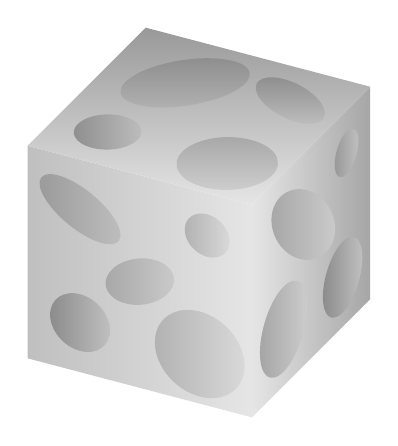
\begin{tikzpicture}[x  = {(0.5cm,0.5cm)},
                    y  = {(0.95cm,-0.25cm)},
                    z  = {(0cm,0.9cm)}]

    \def\a{1.5}

    \begin{scope}[canvas is yz plane at x=-\a]
        \shade[left color=gray!50,right color=gray!20] (-\a,-\a) rectangle (\a,\a);
        \shade[left color=gray!60,right color=gray!30] (0.9,0.9) circle (0.3);
        \shade[left color=gray!60,right color=gray!30] (0.8,-0.8) circle (0.6);
        \shade[left color=gray!90,right color=gray!50] (-0.8,-0.8) circle (0.4);
        \shade[left color=gray!70,right color=gray!40, rotate = 30] (0,0) ellipse (0.5 and 0.3);
        \shade[left color=gray!80,right color=gray!50, rotate around={330:(-0.8,0.8)}] (-0.8,0.8) ellipse (0.6 and 0.3);
    \end{scope}
    \begin{scope}[canvas is xz plane at y=\a]
        \shade[right color=gray!70,left color=gray!20] (-\a,-\a) rectangle (\a,\a);
        \shade[left color=gray!80,right color=gray!50] (0.9,0.9) circle (0.3);
        \shade[left color=gray!90,right color=gray!50] (0.8,-0.8) circle (0.5);
        \shade[left color=gray!70,right color=gray!40] (-0.7,-0.7) circle (0.6);
        %\shade[left color=gray!70,right color=gray!40] (-0.2,0.5) circle (0.6);
        %\shade[left color=gray!40,right color=gray!70, rotate = 30] (0,0) ellipse (0.5 and 0.3);
        \shade[left color=gray!70,right color=gray!40, rotate around={140:(-0.2,0.5)}] (-0.2,0.5) ellipse (1.0 and 0.4);
    \end{scope}
    \begin{scope}[canvas is yx plane at z=\a]
        \shade[top color=gray!80,bottom color=gray!20] (-\a,-\a) rectangle (\a,\a);
        %\shade[left color=gray!60,right color=gray!30] (0.9,0.9) circle (0.3);
        \shade[top color=gray!90,bottom color=gray!50, rotate around={330:(0.8,0.8)}] (0.8,0.8) ellipse (0.6 and 0.3);
        \shade[top color=gray!70,bottom color=gray!40] (0.8,-0.8) circle (0.6);
        \shade[left color=gray!90,right color=gray!50] (-0.8,-0.8) circle (0.4);
        %\shade[left color=gray!70,right color=gray!40, rotate = 30] (0,0) ellipse (0.5 and 0.3);
        \shade[top color=gray!90,bottom color=gray!60, rotate around={50:(-0.5,0.6)}] (-0.5,0.6) ellipse (0.8 and 0.5);
    \end{scope}
\end{tikzpicture}
	\captionof{figure}{Illustration of porous media cude}
	\label{fig:porous-cube}
\end{center}

Many everyday processes involve the flow of a liquid into a porous media [Fig. \ref{fig:porous-cube}], dunking a biscuit into coffee, cleaning the floor with a cloth, or get drenched with rain. The same process is also important in nature for water to reach the tips of the tallest trees or to flow through soil and for different industrial processes, ranging from oil recovery and chromatography to food processing, agriculture, heterogeneous catalysis, and impregnation. The above processes are examples of imbibition. Imbibition of a liquid into a porous media is governed by the interplay of capillary pressure, viscous drag, volume conservation, and gravity. The porous media often has a complex topology, which result in variations in the permeability and in the capillary pressure at the moving interface. Nevertheless, the invasion front during solely capillarity-driven imbibition advances in a simple square root of time manner, according to the "Lucas–Washburn Law"\cite{Bell1906, Lucas1918, Washburn1921}. It is valid down to nanoscopic pore sizes (REFERENCES) and particularly robust with regard to the geometrical complexity of the porous media \cite{Reyssat2008}. The evolution of the invasion front displays universal scaling features on large length and timescales, which are independent of the microscopic details of the fluid and media. \cite{Gruener2012}	

\section{BCLW Imbibition}
\label{sec:BCLW-imbibition}

In this section "BCLW Imbibition" also known as "Lucas-Washburn Law". BCLW stands here for Bell \& Cameron\cite{Bell1906}, Lucas\cite{Lucas1918} and Washburn\cite{Washburn1921} and their contribution to the topic of capillary flow. This part is based on the contribution of Edward W. Washburn\cite{Washburn1921}.

\begin{center}
	\captionsetup{type=figure}
	
% \usetikzlibrary{angles, quotes, calc}

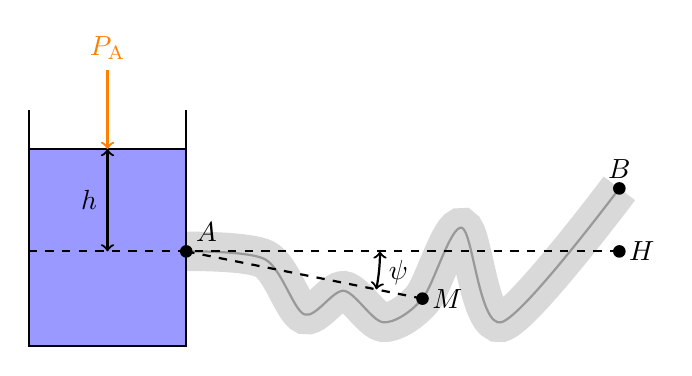
\begin{tikzpicture}

    % Coordinates
    \coordinate (end) at (4,1.2);
    \coordinate (start) at (4,0.8);
    \coordinate (A) at (2,1.2);
    \coordinate (B) at (7.5,2);
    \coordinate (M) at (5,0.6);
    \coordinate (H) at (7.5,1.2);

    % Capillar
    \draw [line width=0.5cm, gray!30] plot [smooth] coordinates { (A) (3,1.1) (3.5,0.4) (4,0.7) (4.5,0.3) (M) (5.5,1.5) (6,0.3) (B)};
    \draw [thick, gray!80] plot [smooth] coordinates { (A) (3,1.1) (3.5,0.4) (4,0.7) (4.5,0.3) (M) (5.5,1.5) (6,0.3) (B)};

    % Glas with Water
    \draw [thick] (0,0) -- (0,3);
    \draw [thick] (2,0) -- (2,3);
    \draw [thick, fill = blue!40] (0,0) rectangle (2,2.5);

    % Horizontal Line and Angle 
    \draw [thick, dashed] (0,1.2) -- (H);
    \draw [thick, dashed] (A) -- (M); %node[below] {$l_\mathrm{s}$}

    \pic [thick, draw, <->, "$\psi$", angle eccentricity=1.1, angle radius = 70] {angle = start--A--end};

    % Air Pressure and Height
    \draw [thick, ->, orange]  (1,3.5) node[above] {$P_\mathrm{A}$} -- (1,2.5);
    \draw [thick, <->] (1,2.5) -- node[left] {$h$} (1,1.2);

    % Point A, B, M
    \fill (A) circle (0.08) node [above right] {$A$};
    \fill (B) circle (0.08) node [above] {$B$};
    \fill (M) circle (0.08) node [right] {$M$};
    \fill (H) circle (0.08) node [right] {$H$};

    

\end{tikzpicture}
	\captionof{figure}{Theoretical set up of BCLW imbibition with atmospheric pressure $\Pa$, depth $h$ and position angle $\psi$.}
	\label{fig:lucas-washburn-setup}
\end{center}

In the following a closer look at a single capillary tube with uniform circular cross-section with radius $r$ and any length and shape which is connected to a glass containing liquid will be made. The tube makes contact with the liquid at point $A$ in a depth of $h$. The end $B$ should either be open to the atmosphere or closed and completely evacuated. A sketch of previous thoughts can be seen in Fig. \ref{fig:lucas-washburn-setup}.
\bigskip

At the beginning the liquid establishes connection with the tube. After some time $t_0$ the meniscus will have penetrated a distance $l_0$ at which point its velocity will have dropped to a value that follows the condition of flow postulated in Poiseuille's law and will thereafter persist. For the dynamics of capillary flow only the Poiseuille region is from concern if the capillaries are chosen small enough. Poiseuille's law with neglected air resistance will then be given by the equation
\begin{gather}
	dV = \frac{\pi \Pt}{8\mu l}\left(r^4 + 4\epsilon r^3 \right) dt~,
	\label{eq:poiseuille-law}
\end{gather}
where $dV$ is the volume of the liquid which in the time $dt$ flows through any cross-section of the capillary, $l$ the length of the column liquid in the capillary at the time $t$, $\mu$ the viscosity of the liquid and $\epsilon$ its coefficient of the slip and $\Pt$ the total driving pressure upon the liquid. The meniscus will have arrived at Point $M$ after the time $t$ with the velocity of $\left(\mathrm{d}l/\mathrm{d}t\right)$. Since the capillary is in cylindrical shape the change of volume $dV$ can also be written as
\begin{gather}
	dV = \pi r^2 dl
	\label{eq:change-cylinder}
\end{gather}
with the circular cross-section $\pi r^2$ and the change of length $dl$. Together with Equation (\ref{eq:poiseuille-law}) results in the following expression for the velocity
\begin{gather}
	\dldt = \frac{\Pt}{8\mu l}\left(r^2 + 4\epsilon r \right)~.
	\label{eq:poiseuille-velocity}
\end{gather}
The total driving pressure $\Pt$ will be made up in three separate pressures, the atmospheric pressure $\Pa$, the hydrostatic pressure $\Ph$ and the capillary pressure $\Ps$. The atmospheric pressure $\Pa$ shall be taken constant. The hydrostatic pressure can be written as
\begin{gather}
	\Ph = hgD - \ls g D \sin \psi~,
	\label{eq:hydrostatic-pressure}
\end{gather}
where $\ls$ is the linear distance from point $A$ to $M$, $g$ the acceleration due to gravity, $D$ the density of the liquid, the depth $h$ and $\psi$ the angle between $\overline{AM}$ and $\overline{AH}$ and will be referred as position angle. For the capillary pressure the following expression is known
\begin{gather}
	\Ps = \frac{2\gamma}{r}\cos \theta~,
	\label{eq:capillary-pressure}
\end{gather}
where $\gamma$ is the surface tension and $\theta$ the contact angle. Summing up the total driving pressure can be written as
\begin{gather}
	\Pt = \left(\Pa + gD (h - \ls \sin \psi) + \frac{2\gamma}{r}\cos \theta\right)~.
	\label{eq:pressure}
\end{gather}
Substuting Equation (\ref{eq:pressure}) into Equation (\ref{eq:poiseuille-velocity}) gives the law for the velocity of penetration as 
\begin{gather}
	\dldt = \frac{\left(\Pa + gD (h - \ls \sin \psi) + \frac{2\gamma}{r}\cos \theta\right)}{8\mu l}\left(r^2 + 4\epsilon r \right)~.
	\label{eq:poiseuille-velocity-pressure}
\end{gather}
The liquid after the distance $l_0$ is then determined by the relation
\begin{gather}
	\frac{2rD}{\mu}\dldt = k~,
	\label{eq:osbourne-reynolds}
\end{gather}
where $k$ is a pure number where experiments found that it is of the order $\sim 10^3$. Combine this relation with Equation (\ref{eq:poiseuille-velocity-pressure}) and assume an position angle $\psi = 0$ the following expression for the distance $l_0$ can be obtained 
\begin{gather}
	l_0 = \frac{\left(\Pa + gDh + \frac{2\gamma}{r}\cos \theta\right) D r^3}{4\mu k}~,
\end{gather}
which states that the distance $l_0$ is entirely negligible for very small capillaries ($l_0 \sim r^3$). 
\bigskip

To determine the length of column liquid $l$ after the time $t$ Equation (\ref{eq:poiseuille-velocity-pressure}) will be rearranged under the assumption $\psi$, $\epsilon$ and $\theta$ are constant and $\ls \approx l$. This results in the following expression
\begin{gather}
	\begin{aligned}
		\dldt &= \frac{\left(r^2 + 4\epsilon r \right)}{8\mu}\frac{\left(\Pa + gDh + \frac{2\gamma}{r}\cos \theta - gDl \sin \psi \right)}{l}\\
			  &= R \frac{\left(\Pt^* - \Ph^* l\right)}{l} = \frac{R \Ph^* \left( 1 - (\Ph^*/\Pt^*) l\right)}{(\Ph^*/\Pt^*) l}~,
	\end{aligned}
	\label{eq:poiseuille-velocity-pressure-rearranged}
\end{gather}
where $\Pt^*$ is the reduced total driving pressure, $\Ph^*$ the reduced hydrostatic pressure coefficient and $R$ a constant. Inverting Equation (\ref{eq:poiseuille-velocity-pressure-rearranged}) and integrate for $l$ gives
\begin{gather}
	R \Ph^* t = - l - \frac{1}{(\Ph^*/\Pt^*)} \ln\left(1- (\Ph^*/\Pt^*) l \right)~.
	\label{eq:length}
\end{gather}
Two limiting cases (I) $\psi = \pi/2$ which corresponds to vertical capillaries with small internal surfaces and (II) $\psi = 0$ which refers to horizontal capillaries offer some special interest. For case (I) the hydrostatic pressure coefficient $\Ph^*$ has the value $gD$. Under the assumption that the liquid is moving under its own capillary pressure ($\Pa + Dgh \ll \frac{2\gamma}{r}\cos \theta$) the reduced total driving pressure equals $\Pt^* \approx \frac{2\gamma}{r}\cos \theta$. Furthermore, the assumption $\epsilon = 0$ will be used which is the case for all liquids which wet the capillary and results in $R = r^2/8\mu$. Then the logarithmic term in Equation (\ref{eq:length}) can be expanded to the second order
\begin{gather}
	\begin{aligned}
		R \Ph^* t &\approx - l + \frac{1}{(\Ph^*/\Pt^*)} \left((\Ph^*/\Pt^*) l + \frac{(\Ph^*/\Pt^*)^2}{2} l^2 \right) \\
				  &= \frac{(\Ph^*/\Pt^*)}{2} l^2~,
	\end{aligned}
	\label{eq:length-expanded}
\end{gather}
which can rearranged as
\begin{gather}
	\boxed{l^2 = \left(\frac{\gamma}{\mu}\frac{\cos \theta}{2}\right)rt}~.
	\label{eq:BCLW-Imbibition}
\end{gather}
Equation (\ref{eq:BCLW-Imbibition}) is also known as "Lucas-Washburn Law" and described the distance $l$ which gets penetrated in the capillary after the time $t$. The same result can be obtained in case (II) with the same assumption and a second integration over the length $l$. The rate can be expressed as
\begin{gather}
	\boxed{\dldt = \frac{r}{\mu} \frac{\gamma}{4l} \cos \theta}~.
	\label{eq:rate}
\end{gather}
The rate at which a liquid penetrates any horizontal capillary (or any capillary with a small surface), under its own capillary pressure is directly proportional to the radius of the capillary, to the cosine of the angle of contact, to the ratio of the surface tension to the viscosity of the liquid and inversely proportional to the length already filled by the liquid. The quantity $(\gamma/\mu (\cos \theta)/2)$ is referred as \textit{penetrativity} and measures the penetrating power of a liquid. 
\bigskip

\begin{center}
	\captionsetup{type=figure}
	% \usetikzlibrary{3d}

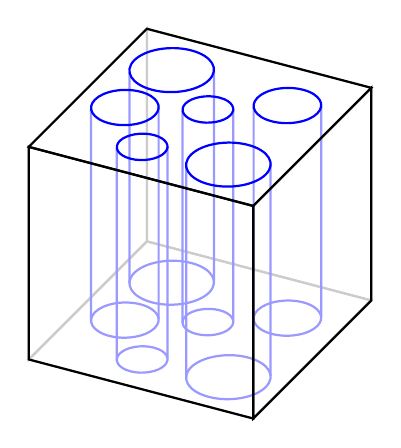
\begin{tikzpicture}[x  = {(0.5cm,0.5cm)},
                    y  = {(0.95cm,-0.25cm)},
                    z  = {(0cm,0.9cm)}]

    \def\a{1.5}

    \begin{scope}[canvas is yz plane at x=\a]
        \draw[thick, gray!34] (-\a,-\a) rectangle (\a,\a);
    \end{scope}
    \begin{scope}[canvas is xz plane at y=-\a]
        \draw[thick, gray!40] (-\a,-\a) rectangle (\a,\a);
    \end{scope}
    \begin{scope}[canvas is yx plane at z=-\a]
        \draw[thick, gray!40] (-\a,-\a) rectangle (\a,\a);
        
        \coordinate (A') at (0.8,-0.8);
        \coordinate (B') at (0.8,0.7);
        \coordinate (c') at (0.0,0.2);
        \coordinate (D') at (-0.8,0.8);
        \coordinate (E') at (-0.9,-0.2);
        \coordinate (F') at (-0.3,-0.9);

        \draw[thick, blue!40] (A') circle (0.5);
        \draw[thick, blue!40] (B') circle (0.4);
        \draw[thick, blue!40] (c') circle (0.3);
        \draw[thick, blue!40] (D') circle (0.5);
        \draw[thick, blue!40] (E') circle (0.4);
        \draw[thick, blue!40] (F') circle (0.3);

    \end{scope}
    
    \begin{scope}[canvas is yx plane at z=\a]

        \coordinate (A) at (0.8,-0.8);
        \coordinate (B) at (0.8,0.7);
        \coordinate (c) at (0.0,0.2);
        \coordinate (D) at (-0.8,0.8);
        \coordinate (E) at (-0.9,-0.2);
        \coordinate (F) at (-0.3,-0.9);

        \draw[thick,blue!40] ($ (A') + (210:0.5) $) -- ($ (A) + (210:0.5) $) ;
        \draw[thick,blue!40] ($ (B') + (210:0.4) $) -- ($ (B) + (210:0.4) $) ;
        \draw[thick,blue!40] ($ (c') + (210:0.3) $) -- ($ (c) + (210:0.3) $) ;
        \draw[thick,blue!40] ($ (D') + (210:0.5) $) -- ($ (D) + (210:0.5) $) ;
        \draw[thick,blue!40] ($ (E') + (210:0.4) $) -- ($ (E) + (210:0.4) $) ;
        \draw[thick,blue!40] ($ (F') + (210:0.3) $) -- ($ (F) + (210:0.3) $) ;

        \draw[thick,blue!40] ($ (A') + (30:0.5) $) -- ($ (A) + (30:0.5) $) ;
        \draw[thick,blue!40] ($ (B') + (30:0.4) $) -- ($ (B) + (30:0.4) $) ;
        \draw[thick,blue!40] ($ (c') + (30:0.3) $) -- ($ (c) + (30:0.3) $) ;
        \draw[thick,blue!40] ($ (D') + (30:0.5) $) -- ($ (D) + (30:0.5) $) ;
        \draw[thick,blue!40] ($ (E') + (30:0.4) $) -- ($ (E) + (30:0.4) $) ;
        \draw[thick,blue!40] ($ (F') + (30:0.3) $) -- ($ (F) + (30:0.3) $) ;

        \draw[thick, blue] (A) circle (0.5);
        \draw[thick, blue] (B) circle (0.4);
        \draw[thick, blue] (c) circle (0.3);
        \draw[thick, blue] (D) circle (0.5);
        \draw[thick, blue] (E) circle (0.4);
        \draw[thick, blue] (F) circle (0.3);
        
        \draw[thick] (-\a,-\a) rectangle (\a,\a);
    \end{scope}
    \begin{scope}[canvas is yz plane at x=-\a]
        \draw[thick] (-\a,-\a) rectangle (\a,\a);
    \end{scope}
    \begin{scope}[canvas is xz plane at y=\a]
        \draw[thick] (-\a,-\a) rectangle (\a,\a);
    \end{scope}

\end{tikzpicture}

	\captionof{figure}{Illustration of the assumption that porous media contains multiple cylindrical capillaries with different radii}
	\label{fig:porous-cube-cylinder}
\end{center}

To calculate the amount of liquid which will have entered the porous body at the end of time $t$ one assumes that the penetration of the pores of a body is equivalent to the penetration of n cylindrical capillary tubes of radii ${r_1,...,r_N}$ [Fig. \ref{fig:porous-cube-cylinder}]. The volume for small capillaries will be together with Equation (\ref{eq:BCLW-Imbibition}) given by
\begin{gather}
	V = \sum_{i=1}^N \pi r_i^2 l = \frac{\pi}{2} \left(\frac{t}{\mu}\right)^{1/2} \sum_{i=1}^N \left(\frac{2 \gamma}{r_i}\cos\theta \right)^{1/2} r_i^3~,
\end{gather}
which can also be written as
\begin{gather}
	\boxed{V = k \left(\frac{\gamma}{\mu}\right)^{1/2} t^{1/2}}~, 
	\label{eq:volume-cylinder}
\end{gather}
where $k$ is independent of the nature of the liquid. Finally, the degree of penetration is proportional to the square root of the ratio of surface tension to the viscosity. For nanoscopic pores Equation (\ref{eq:volume-cylinder}) still applies (REFERENCES). Equation (\ref{eq:volume-cylinder}) can only be applied for pores with no enlargement or pocket at the ends and no changes of the cross-section of a pore with its length. The latter case will be discussed in the next paragraph.

\section{Imbibition in Geometries with Axial Variations}
\label{sec:geometry}

In this paragraph the influence of the capillary geometry on the imbibition dynamics will be studied. This section is based on the publication from Reyssat et al. \cite{Reyssat2008}. In the following only the three-dimensional case will be discussed.
\bigskip

To characterize the viscous dominated dynamics the incompressible flows will be treated as one-dimensional in the axial or z-direction while using the classical Darcy description. The analytical development is general for any one-dimensional flow to which the Darcy description applies. $r(z)$ donates here half of the width of the capillary and $z = 0$ indicates the opening with radius $r(0) = r_0$. Figure \ref{fig:geometry} shows three different geometry in two-dimensional plane where (a) cylindrical, (b) cone and (c) parabolic capillary. These capillaries are in contact with a reservoir of liquid at ambient pressure $P_0$, containing atmospheric pressure $\Pa$ and hydrostatic pressure $\Ps$. Wetting of the liquid on the walls leads to an invasion process.

\begin{center}
	\captionsetup{type=figure}
	% \usetikzlibrary{angles, quotes, calc}

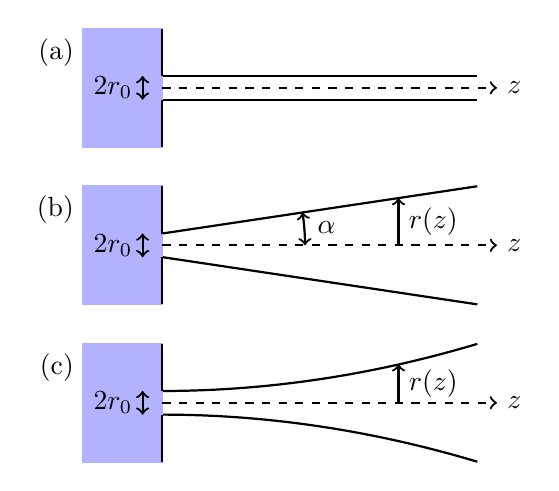
\begin{tikzpicture}

    % Coordinates
    \coordinate (A) at (0, 2.75);
    \coordinate (start) at (5.25, 2.75);
    \coordinate (end) at (5,3.5);

    % Capillar
    % Cylinder
    \draw [thick] (1,4.9) -- (5,4.9);
    \draw [thick] (1,4.6) -- (5,4.6);
    % Wedge
    \draw [thick] (1,2.9) -- (5,3.5);
    \draw [thick] (1,2.6) -- (5,2.0);
    % Parabolic
    \draw [thick, domain = 0:8, variable = \x] plot ({4/8 * \x + 1}, {- \x*\x /107 + 0.6});
    \draw [thick, domain = 0:8, variable = \x] plot ({4/8 * \x + 1}, {+ \x*\x /107 + 0.9});

    % Glas with Water
    % Parabolic
    \draw [thick, fill = blue!30!white, blue!30!white] (0,0) rectangle (1,1.5);
    \draw (0,1.5) node [below left] {(c)};
    \draw [thick] (1,0.9) -- (1,1.5);
    \draw [thick] (1,0.0) -- (1,0.6);
    % Wedge
    \draw [thick, fill = blue!30!white, blue!30!white] (0,2) rectangle (1,3.5);
    \draw (0,3.5) node [below left] {(b)};
    \draw [thick] (1,2.9) -- (1,3.5);
    \draw [thick] (1,2.0) -- (1,2.6);
    % Cylinder
    \draw [thick, fill = blue!30!white, blue!30!white] (0,4) rectangle (1,5.5);
    \draw (0,5.5) node [below left] {(a)};
    \draw [thick] (1,4.9) -- (1,5.5);
    \draw [thick] (1,4.0) -- (1,4.6);

    % Z-Axis
    \draw [thick, ->, dashed] (1, 4.75) -- (5.25, 4.75) node [right] {$z$};
    \draw [thick, ->, dashed] (1, 2.75) -- (5.25, 2.75) node [right] {$z$};
    \draw [thick, ->, dashed] (1, 0.75) -- (5.25, 0.75) node [right] {$z$};

    % r0 
    \draw [thick, <->] (0.75,4.6) -- node [left] {$2r_0$} (0.75,4.9);
    \draw [thick, <->] (0.75,2.6) -- node [left] {$2r_0$} (0.75,2.9);
    \draw [thick, <->] (0.75,0.6) -- node [left] {$2r_0$} (0.75,0.9);

    % Angle 
    \pic [thick, draw, <->, "$\alpha$", angle eccentricity=1.1, angle radius = 80] {angle = start--A--end};

    % r(z)
    \draw [thick, ->] (4, 2.75) -- node [right] {$r(z)$} (4, 3.35) ;
    \draw [thick, ->] (4, 0.75) -- node [right] {$r(z)$} (4, 1.24);

\end{tikzpicture}
	\captionof{figure}{Different geometries for illustrating variants of the capillary-driven invasion of a structured porous solid with axial shape variations: (a) straight (b) conical (c) parabolic capillary. $r_0$ and $r(z)$ are the radius of the opening and at the distance $z$ and $\alpha$ is here the opening angle. The capillaries are in contact with a fluid reservoir on the left with pressure $P_0$.}
	\label{fig:geometry}
\end{center}

The averaged velocity is $u$ is assumed to be in the form of Darcy's law,
\begin{gather}
	\frac{\mu u}{k} = -\frac{\partial \Pt}{\partial z}~,
	\label{eq:darcy-law}
\end{gather}
where $k$ is the permeability, which depends on the detailed shape of the cross-section. For slowly varying nearly rectangular shapes $k$ can be written as
\begin{gather}
	k = \frac{r(z)^2}{\lambda} = \frac{r(z)^2}{8}
	\label{eq:permeability}
\end{gather}
In addition to that mass conservation states that volumetric flow rate $Q$ is given by
\begin{gather}
	Q = u \pi r(z)^2  
	\label{eq:volume-flux}
\end{gather}
Furthermore, assume that the meniscus of the liquid is a $z = l$ and the total driving pressure at that point is given by $\Pt = P_0 - c \gamma/r(z)$, where $c$ depends on the local geometry and the contact angle $\theta$ the liquid makes with the solid. Inserting Equation (\ref{eq:permeability}) and (\ref{eq:volume-flux}) into Darcy's law yields
\begin{gather}
	\frac{8 \mu Q}{\pi r(z)^4} = -\frac{\partial \Pt}{\partial z}~,
	\label{eq:darcy-law-flux}
\end{gather}
which gets integrated from $z=0$ ($\Pt = P_0$) and $z = l$ ($\Pt = P_0  - c \gamma/r(l)$) and results in the expression for the flow rate $Q$ given by
\begin{gather}
	Q = \frac{c \pi \gamma}{8\mu} \left[ r(l) \int_0^{l}\!\!\!\dz~r(z)^{-4} \right]^{-1}~.
	\label{eq:volume-flux-integral}
\end{gather}
The rate of penetration $\left(\mathrm{d}l/\mathrm{d}t\right)$ is then given by the speed of the movement $u_\mathrm{m}$ of the meniscus as $u_\mathrm{m} = \left(\mathrm{d}l/\mathrm{d}t\right) = Q / (\pi r(l)^2)$, resulting in the relation
\begin{gather}
	\boxed{\dldt = \frac{c \gamma}{8\mu} \left[ r(l)^3 \int_0^{l}\!\!\!\dz~r(z)^{-4} \right]^{-1}}~.
	\label{eq:rate-geometry}
\end{gather}
Equation (\ref{eq:rate-geometry}) serves as generalization of the usual imbibition equation for invasion into a structured (shaped) solid in three dimension.
\bigskip

In the next step the general case of a power-law-shaped profile will be considered to solve Equation (\ref{eq:rate-geometry}) and is given by
\begin{gather}
	r(z) = r_0 + \alpha z^n~,
	\label{eq:power-law}
\end{gather}
where $\alpha$ is the opening angle and depends on the exponent $n$. Then the meniscus motion can be expressed as 
\begin{gather}
	\dldt = \frac{c \gamma r_0}{8\mu} \left[ \left(1 + \frac{\alpha}{r_0} l^n \right)^3 \int_0^{l}\!\!\!\dz~\left(1 + \frac{\alpha}{r_0} z^n \right)^{-4} \right]^{-1}~.
	\label{eq:rate-geometry-power-law}
\end{gather}
In general $c$ depends on the position of the meniscus and the geometry with $c(l) = 2\cos(\theta + \arctan(\mathrm{d}r/\mathrm{d}z(l)))$ but since the cosine is bounded the approximation of $c = \text{const}$ will be made. Additionally, to preserve clarity the following dimensionless parameters will be introduced
\begin{gather}
	L = \left(\frac{\alpha}{r_0}\right)^{1/n} l\quad\text{and}\quad T = \frac{c\gamma r_0}{8\mu} \left(\frac{\alpha}{r_0}\right)^{2/n} t~,
\end{gather}
which reduces Equation (\ref{eq:rate-geometry-power-law}) to
\begin{gather}
	\dLdT = \left[ \left(1 + L^n \right)^3 \int_0^{L}\!\!\!\dZ~\left(1 + Z^n \right)^{-4} \right]^{-1}~.
	\label{eq:rate-geometry-power-law-reduced}
\end{gather}
Equation (\ref{eq:rate-geometry-power-law-reduced}) has two cases:\\
(I) For $n = 0$ ($r(z) = r_0$) the known "Lucas-Washburn Law" from paragraph \ref{sec:BCLW-imbibition} can be recovered from Equation (\ref{eq:rate-geometry-power-law-reduced}).\\
 (II) For $n > 1$ there are two asymptotic limits to identify:\\
(i) At short times, which corresponds to $L \ll 1$ and $\int_0^{L}\!\dZ~\left(1 + Z^n \right)^{-4} \simeq L$. Thus, Equation (\ref{eq:rate-geometry-power-law-reduced}) simply into
\begin{gather}
	L \dLdT \simeq \text{const}~ \Rightarrow \boxed{L \sim T^{1/2}}
\end{gather}
which can be identified as the classical "Lucas-Washburn Law".\\
(ii) At long times, or when $L \gg 1$, $(1+L^n) \simeq L^n$ and the integral $\int_0^{L}\!\!\!\dZ~\left(1 + Z^n \right)^{-4} \simeq L$ can be approximate by $\int_0^{\infty}\!\dZ~\left(1 + Z^n \right)^{-4} \simeq L$, which converge if $n > 1/4$ to a constant value. Thus, Equation (\ref{eq:rate-geometry-power-law-reduced}) become
\begin{gather}
	L^{3n} \dLdT \simeq \text{const}~\Rightarrow \boxed{L \sim T^{1/(3n+1)}}~.
\end{gather}
To conclude independent of the shape of the capillary for short times the "Lucas-Washburn Law" ($L \sim T^{1/2}$) still applies but for long times a different dynamic ($L \sim T^{1/(3n+1)}$) have to be considered resulting in two regimes. The cross-over between these two limits occurs for $L \simeq 1$, i.e. $l \simeq (r_0/\alpha)^{1/n}$ and since the second regime depends on the parameter $n$, i.e. the shape of the capillary, one finally say that the more diverging the geometry, the slower the dynamics become at long times.  In Fig. \ref{fig:geometry-dynamics}, three different solutions of Equation (\ref{eq:rate-geometry-power-law-reduced}) have been represented for the three-dimensional axisymmetric geometry. For each value of $n$ the former regimes are clearly visible.
\begin{center}
	\captionsetup{type=figure}
	\includegraphics[width = \linewidth]{../pictures/Geometry-Dynamics.png}
	\captionof{figure}{
		Log-log representation of analytical solutions of Equation (\ref{eq:rate-geometry-power-law-reduced}) for three values of $n$ in the three-dimensional axisymmetric geometry. $L$ and $T$ are, respectively, the dimensionless position of the meniscus and time. The "Lucas-Washburn Law" $L \sim T^{1/2}$ is represented by the continuous line. The more diverging the geometry the slower the dynamics is at long times.
	}
	\label{fig:geometry-dynamics}
\end{center}

\section{Imbibition Experiments}


% BIBLIOGRAPHY =============================================================================================================

%\nocite{*}
\bibliography{references.bib}% Produces the bibliography via BibTeX.

\end{document}
% END MAIN =================================================================================================================
% ****** End of file aipsamp.tex ******
